\section{Implementations-Sicht}
\label{sec:sad-implementation}

\subsection{Rendering des User Interfaces und Event-Behandlung}
Durch die Verwendung von \emph{barefoot} \cite{Barefoot} kann die komplette Beispielapplikation sowohl eigenständig auf dem Server gerendert werden, als auch als moderne JavaScript Applikation im Browser des Endbenutzers ausgeführt werden. Aus diesem Grund zeigen die folgenden zwei Abschnitte jeweils ein separates Sequenzdiagramm: Eines für das Event-Handling auf dem Client und eines für den Rendering-Vorgang auf dem Server.

Grundlegende Unterschiede gibt es hierbei lediglich beim Zugriff auf den \emph{APIAdapter}. Auf dem Server werden diese direkt lokal behandelt, im Client-Browser wird die entsprechende API-Abfrage über einen HTTP \gls{REST} Request übertragen.

\subsubsection*{Server}
Beim initialen Aufruf der Beispielapplikation werden die kompletten Inhalte des User Interfaces auf dem Server gem. Diagramm \ref{dig:serverrendering} gerendert. Sollte der Client-Browser zudem JavaScript deaktiviert haben oder nicht unterstützen, so werden auch nachfolgende Requests nach dem gleichen Schema verarbeitet und gerendert.

\begin{figure}[H]
	\centering{
		\resizebox{0.9\textwidth}{!} {
			\begin{tikzpicture}
				\begin{umlseqdiag}
					\umlactor[class=Browser, fill=white]{client}
					\umlboundary[class=ExpressJS, fill=white]{app}
					\umlobject[class=Router, fill=sharedColor!20]{router}
					\umlobject[class=View, fill=sharedColor!20]{view}
					\umlobject[class=Model, fill=sharedColor!20]{model}
					\umlobject[class=ApiAdapter, fill=apiColor!20]{apiAdapter}
					\umlobject[class=DataStore, fill=barefootColor!20]{dataStore}

					\begin{umlcall}[op={Click -> Request}, return=HTML]{client}{app}
						\begin{umlcall}[op=route(), with return]{app}{router}
							\begin{umlcallself}[op=render()]{router}
								\begin{umlcallself}[op=initDOM()]{router}
								\end{umlcallself}
								\begin{umlcallself}[op=renderMainView()]{router}
								\end{umlcallself}

								\begin{umlcallself}[op=renderView()]{router}
									\begin{umlcall}[op=beforeRender(), with return]{router}{view}
										\begin{umlcall}[op={fetch()}, return=success()]{view}{model}
											\begin{umlcall}[op={sync()}, return=success()]{model}{apiAdapter}
											\end{umlcall}
										\end{umlcall}
									\end{umlcall}

									\begin{umlcall}[op=renderView(), return=HTML]{router}{view}
									\end{umlcall}

									\begin{umlcall}[op=afterRender(), with return]{router}{view}
									\end{umlcall}
								\end{umlcallself}

								\begin{umlcall}[op=toJSON(), with return]{router}{dataStore}
								\end{umlcall}

								\begin{umlcallself}[op=writeHTTPResponse()]{router}
								\end{umlcallself}
							\end{umlcallself}
						\end{umlcall}
					\end{umlcall}
				\end{umlseqdiag}
			\end{tikzpicture}
		}
	}
	\caption{Sequenzdiagramm: Rendering und Event-Verarbeitung auf dem Server}
	\label{dig:serverrendering}
\end{figure}

\subsubsection*{Client}
Das Sequenzdiagramm \ref{dig:clientrendering} zeigt den Kontrollfluss nachdem der Benutzer im Browser auf einen Eintrag im Navigationsmenü geklickt hat.

Es gilt zu beachten, dass die Aufrufe auf den \emph{APIAdapter} nicht lokal sondern direkt auf dem Server verarbeitet werden.

\begin{figure}[H]
	\centering{
		\resizebox{0.9\textwidth}{!} {
			\begin{tikzpicture}
				\begin{umlseqdiag}
					\umlactor[class=Browser]{client}
					\umlobject[class=View]{current}
					\umlobject[class=Router]{router}
					\umlobject[class=View]{next}
					\umlobject[class=Model]{model}
					\umlobject[class=Backbone]{backbone}
					\umlobject[class=ApiAdapter]{apiAdapter}

					\begin{umlcall}[op=Click Menu Item, with return]{client}{current}
						\begin{umlcall}[op=navigate(), with return]{current}{router}
							\begin{umlcallself}[op=render()]{router}
								\begin{umlcallself}[op=renderView()]{router}
									\begin{umlcall}[op=beforeRender(), with return]{router}{next}
										\begin{umlcall}[op={fetch()}, return=success()]{next}{model}
											\begin{umlcall}[op={sync()}, return=success()]{model}{backbone}
												\begin{umlcall}[op={HTTP REST Request}, return=HTTP Response]{backbone}{apiAdapter}
												\end{umlcall}
											\end{umlcall}
										\end{umlcall}
									\end{umlcall}

									\begin{umlcall}[op=renderView(), return=HTML]{router}{next}
									\end{umlcall}

									\begin{umlcall}[op=afterRender(), with return]{router}{next}
									\end{umlcall}
								\end{umlcallself}

								\begin{umlcallself}[op=Replace DOM Element]{router}
								\end{umlcallself}
							\end{umlcallself}
						\end{umlcall}
					\end{umlcall}
				\end{umlseqdiag}
			\end{tikzpicture}
		}
	}
	\caption{Sequenzdiagramm: Rendering und Event-Verarbeitung auf dem Client}
	\label{dig:clientrendering}
\end{figure}



\subsection{APIAdapter}
Wie bereits erwähnt kann der \emph{APIAdapter} auf dem Server sowohl mit server-lokalen Requests als auch mit HTTP REST Anfragen umgehen.

Das Diagramm \ref{dig:apiAdapter} verdeutlicht die Abläufe im innern des Adapters für den jeweiligen Anfragemodus.

Hinter dem Element \emph{Controllers} stehen neben dem eigentlichen API-Controller zusätzlich diverse Sicherheitspolicies und Validatoren, welche eingehende Requests prüfen und ggf. abweisen können, bevor sie zur eigentlichen Geschäftslogik gelangen.

\begin{figure}[H]
	\centering{
		\resizebox{0.9\textwidth}{!} {
			\begin{tikzpicture}
				\begin{umlseqdiag}
					\umlactor[class=Caller]{caller}
					\umlboundary[class=ExpressJS]{app}
					\umlobject[class=APIAdapter]{apiAdapter}
					\umlmulti[class=Controllers]{controller}
					\umldatabase[class=Persistency]{db}

					\begin{umlfragment}[type=alt, label={Server-local}, inner xsep=12]
						\begin{umlcall}[op={sync()}, return={success()}, dt=8]{caller}{apiAdapter}
							\begin{umlcallself}[op={dispatchLocalApiCall()}]{apiAdapter}
							\end{umlcallself}
							\begin{umlcallself}[op={processCallbacks()}]{apiAdapter}
							\end{umlcallself}
							\begin{umlcall}[op={handler()}, return={success()}]{apiAdapter}{controller}
								\begin{umlcall}[op={consume}, with return]{controller}{db}
								\end{umlcall}
							\end{umlcall}
						\end{umlcall}

						\umlfpart[HTTP REST]

						\begin{umlcall}[op={HTTP Request}, return={JSON Response}]{caller}{app}
							\begin{umlcallself}[op={Dispatch}]{app}
							\end{umlcallself}
							\begin{umlcall}[op={handler()}, return={JSON Object}]{app}{apiAdapter}
								\begin{umlcallself}[op={processCallbacks}]{apiAdapter}
								\end{umlcallself}
								\begin{umlcall}[op={handler()}, return={success()}]{apiAdapter}{controller}
									\begin{umlcall}[op={consume}, with return]{controller}{db}
									\end{umlcall}
								\end{umlcall}
							\end{umlcall}
						\end{umlcall}
					\end{umlfragment}

				\end{umlseqdiag}
			\end{tikzpicture}
		}
	}
	\caption{Sequenzdiagramm: APIAdapter im server-lokalen sowie HTTP REST Modus}
	\label{dig:apiAdapter}
\end{figure}

\newpage

\subsection{Quellcode Organisation}
Für Applikationen mit \gls{nodejs} ist es üblich (\cite{TJH_ComponentStructure}, \cite{IZS_ComponentStructure}), den Quellcode soweit wie möglich eigenständige Komponenten zu unterteilen.

Ein gutes Beispiel hierfür ist die Vielzahl an verfügbaren Modulen welche über den Komponentenmanager NPM \cite{NPM} installierbar sind. Selbst Bibliotheken mit minimalem Umfang werden und sollten als eigene Module gekapselt werden.

Die Beispielapplikation \emph{Roomies} verwendet mehrere Komponenten aus NPM (siehe Quelltext \ref{lst:roomiesPackageJson}) und ist dabei selbst in Komponenten unterteilt. Die Ordnerstruktur in Abbildung \ref{fig:roomiesFolderStructure} veranschaulicht dieses Prinzip.

\begin{lstlisting}[language=JavaScript, firstnumber=9, caption={Auszug der verwendeten NPM Komponenten \cite{RoomiesPackageJson}}, label={lst:roomiesPackageJson}, float=ht!]
, "dependencies": {
	"debug": "~0.7.2"
	, "express": "~3.1.0"
	, "sqlite3": "~2.1.7"
	, "pg": "~0.15.1"
	, "sequelize": "git://github.com/mweibel/sequelize.git#mekanics-mweibel-fix"
	, "node-barefoot": "~0.0.11"
\end{lstlisting}

\begin{figure}[H]
	\centering
	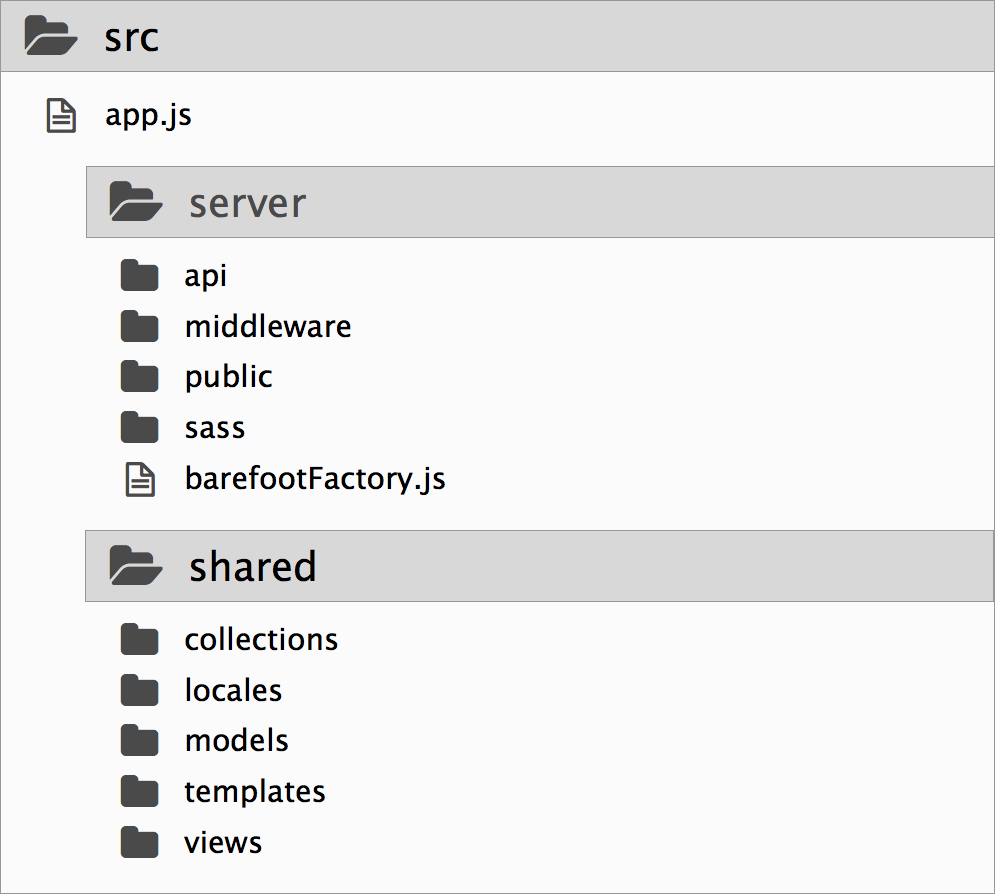
\includegraphics[width=8cm]{content/sad/images/folder-structure.png}
	\caption{Ordnerstruktur des \emph{src}-Unterordners der Beispielapplikation \emph{Roomies}}
	\label{fig:roomiesFolderStructure}
\end{figure}

Jede Komponente mit JavaScript-Code kann mittels einem \emph{require()}-Befehl eingebunden werden womit automatisch die enthaltene \emph{index.js}-Datei geladen wird.

\newpage
\begin{lstlisting}[language=JavaScript, caption=Einbindung der Community-Komponente]
// Requires actually src/server/api/community/index.js:
// Found in src/server/api/index.js
var setupCommunityApi = require('./community');
\end{lstlisting}

Im Folgenden werden die beiden wichtigsten Dateien für das Starten der Applikation erklärt.

\subsubsection*{barefootFactory.js}
Die ``barefoot''-Factory \cite{barefootFactoryjs} ist verantwortlich für das Setup der Server-Seite der Applikation.
Unter anderem werden folgende wichtige Aufgaben ausgeführt:
\begin{itemize}
	\item Definieren der JavaScript Dateien, welche zum Client übertragen werden sollen
	\item Einrichten des API-Adapters
	\item Express.js \cite{Expressjs} Middlewares laden und initialisieren
	\item Express.js \cite{Expressjs} HTTP Server starten
	\item Einrichten des Server Request Contexts (u.a. das Model für den eingeloggten Benutzer)
\end{itemize}

Diese Informationen werden ``barefoot'' \cite{Barefoot} mitgegeben, damit das Framework weiss, was zu starten ist.

\subsubsection*{app.js}
Die Datei ``app.js'' \cite{appjs} ist der Startpunkt der Applikation.
Darin wird u.a. die ``barefootFactory'' instanziert und der ``DataStore'' initialisiert.

Der ``DataStore'' ist ein ``barefoot''-Konzept \cite{barefootDatastore}. Es wird verwendet um Models und Collections vom Server zum Client zu senden.

\newpage
\subsection{Barefoots Mixin Technik}

\emph{Barefoot} \cite{Barefoot} ermöglicht die Verwendung desselben \emph{Backbone.js} Quelltexts sowohl auf dem Server als auch auf dem Client. Dies wird durch gezieltes Einsetzen von Codefragmenten mittels \gls{Mixin}s erreicht.

Dazu werden neutrale Versionen jeder \emph{barefoot}-Komponente während der Initialisierung des Frameworks (siehe Quelltext \ref{lst:BarefootDetermineRuntimeEnvironment}) mit umgebungsspezifischen Mixins ergänzt.

\begin{lstlisting}[language=JavaScript, firstnumber=68, caption={Ermittlung der Runtime-Umgebung sowie anschliessendes applizieren der spezifischen \glspl{Mixin} \cite{BarefootDetermineRuntimeEnvironment}}, label={lst:BarefootDetermineRuntimeEnvironment}, escapeinside={@}{@}]
function boot(options) {
	var Backbone = require('backbone')
		, util = require('./util')
		, environment = options.environment
		@\label{lst:BarefootDetermineRuntimeEnvironment_load}@, mixins = util.loadMixins(environment)
		@\label{lst:BarefootDetermineRuntimeEnvironment_applyMixins}@, Router = require('./router')(mixins.RouterMixin)
		, View = require('./view')(mixins.ViewMixin)
\end{lstlisting}

Sobald die spezifischen \gls{Mixin}s (Zeile \ref{lst:BarefootDetermineRuntimeEnvironment_load}) geladen wurden, werden diese anschliessend ab Zeile \ref{lst:BarefootDetermineRuntimeEnvironment_applyMixins} auf die neutralen Vorlagen appliziert.



\subsection{JavaScript Callbacks}
Insbesondere, aber nicht nur, ein Problemfeld von JavaScript betrifft die Strukturierung von verschachtelten Callback-Funktionen.

Während der Implementation der API für \emph{Roomies} stellte sich wiederholt die Frage, wie asynchron ausgeführter Quelltext am besten strukturiert werden sollte.

\begin{lstlisting}[language=JavaScript, firstnumber=136, caption={Ausschnitt aus Community Controller mit Callback Hell \cite{milestone7CommunityController}}, label={lst:callbackHell}]
function createCommunity(req, res) {
	var resident = req.user
		, db = req.app.get('db')
		, Community = db.daoFactoryManager.getDAO('Community')
		, communityData = {
			name: req.param('name')
		};
	createUniqueShareLink(db, function(err, link) {
		if (err) {
			return res.send(500);
		}
		communityData.shareLink = link;

		resident.getCommunity()
			.success(function getSuccess(community) {
				if (community && community.enabled) {
					req.flash('error',
						res.__('What exactly are you trying? You\'re ' +
							'already in a community...'));
					return res.redirect('/community');
				}

				Community.find({ where: { name: communityData.name }})
					.success(function findResult(community) {
						// ... more callbacks (see cited file)
					})
					.error(function findError() {
						return res.send(500);
					});
			})
			.error(function getError() {
				return res.send(500);
			});
	});
}
\end{lstlisting}

Quelltext \ref{lst:callbackHell} zeigt einen Ausschnitt der \emph{createCommunity}-Funktion. Es ist offensichtlich, dass dieser Quelltext aufgrund der Verschachtlung von Funktionen sehr schwer lesbar ist. Diese Situation wird treffend als ``\emph{Callback hell}'' bezeichnet.
\\ \\
Für ein Refactoring können folgende zwei Ansätze angewendet werden:

\begin{itemize}
	\item Funktional
	\item Promises / Futures
\end{itemize}

\subsubsection*{Funktional}
Der funktionale Ansatz versucht Callbacks in eigene Funktionen auszulagern und dabei Seiteneffekte zu vermeiden.

Die Vermeidung von Seiteneffekten ist wichtig und wünschenswert, bedingt aber meist die Übergabe vieler einzelner Argumente beim Aufruf der ausgelagerten Funktion.

Quelltext \ref{lst:callbackHellFunctional} zeigt einen Ausschnitt der überarbeiteten Version von Quelltext \ref{lst:callbackHell}. Es wurde der funktionale Ansatz für das Refactoring gewählt.

\begin{lstlisting}[language=JavaScript, firstnumber=192, caption={Ausschnitt aus dem neusten Community Controller \cite{masterCommunityController}}, label={lst:callbackHellFunctional}]
function createCommunity(success, error, data) {
	var // ...
		, forwardError = function forwardError(err) {
			// ...
		}
		, afterCommunitySearch = function afterCommunitySearch(community) {
			// ...
			communityDao.create(communityData)
				.success(afterCommunityCreate)
				.error(forwardError);
		}
		, afterCommunityCreate = function afterCommunityCreate(community) {
			// ...
			createUniqueSlug(db, community.name, community.id
				, function(err, slug) {
					// ...
					community.save()
						.success(afterUpdateCommunitySlug)
						.error(forwardError);
				});
		}
		, afterUpdateCommunitySlug =
			function afterUpdateCommunitySlug(community) {
				// ...

				updateResidentsCommunityMembership(
					resident
					, community
					, function(err) {
						// ...
					}
				);
		};

	createUniqueShareLink(db, function(err, shareLink) {
		// ...
		communityDao.find({ where: { name: communityData.name, enabled: true }})
			.success(afterCommunitySearch)
			.error(forwardError);
	});
}
\end{lstlisting}

Zwar ist der resultierende Quelltext um einiges klarer und einfacher interpretierbar, jedoch führt diese Strukturierung bei jedem Laufzeit-Durchlauf zu einer Neudefinition und -initialisierung der beinhalteten Funktionen.

Der folgende Abschnitt zeigt wie die Problematik \emph{Callback Hell} auf eine andere und potentiell leistungsstärkere Weise gelöst werden kann.


\subsubsection*{Promises / Futures}

In \emph{barefoot} sind mehrere Schritte notwendig, um eine \emph{View} zu rendern (siehe Diagramm \ref{dig:serverrendering}).
Jeder Funktionsaufruf wird asynchron ausgeführt, muss die definierte Ausführungs-Reihenfolge aber unter allen Umständen einhalten.

\emph{Barefoot} verwendet zu diesem Zweck Promises, ein Pattern auch bekannt als \emph{Futures} \cite{FuturesAndPromises}. Die frei zugängliche \emph{Promises}-Spezifikation \cite{PromisesAPlusSpec} wird dabei nicht selbst implementiert sondern von der Bibliothek \emph{Q} \cite{QLibrary} umgesetzt.

\newpage
Quelltext \ref{lst:barefootRouterRenderWithQ} zeigt wie \emph{barefoot} Promises einsetzt.

\begin{lstlisting}[language=JavaScript, firstnumber=215, caption={Ausschnitt aus server/router-mixin.js \cite{barefootRouterRenderWithQ}}, label={lst:barefootRouterRenderWithQ}]
	Q.fcall(initDOM)
	.then(renderMainView)
	.then(renderView)
	.then(serializeDataStore)
	.done(writeHTTPResponse, writeHTTPError);
\end{lstlisting}

Unter Verwendung von Promises wird der Kontrollfluss zentral an einer Stelle gesteuert. Beim funktionalen Refactoring werden diese über mehrere Funktionen verteilt wodurch das Nachvollziehen des Kontrollflusses erschwert wird. Zusätzlich entfällt die erwähnte Neudefinition jeglicher Funktionen bei korrekter Umsetzung.
\\ \\
Beide vorgestellten Refactoring-Methoden bieten eine klare Verbesserung der Les- und Wartbarkeit des Quelltexts. Promises können dabei unter Umständen konzeptuell schwerer greifbar sein als das funktionale Gegenstück, bieten dafür aber den Vorteil des zentral gesteuerten Kontrollflusses.

Es kann und sollte pragmatisch entschieden werden, in welcher Situation welches Vorgehen angebrachter ist.